\begin{comment}
    Short description of what tabular methods are.
     - They keep the value function in a table
     - Discreet states and actions

    Explain k-armed bandit agent from previous chapter.

    Upper confidence bound

    Dynamic programming

    Monte carlo methods

    Temporal difference
     - Sarsa
     - Expected Sarsa
     - Q-learning
     - Double Q-learning

    n-step bootstrapping

    Planning and learning (maybe not)
     - models and planning
     - dyna

    Policy gradient
    
    Working example(s)
     - Discreet state and action space
     - model
       • quadcopter navigation
       • pole
       • some other thing I haven't made yet

\end{comment}

% The action-value function estimate $Q_t(s, a)$ holds the current estimate of the real action-value function $q_*(a)$. If the \gls{rl}-agent is to achieve it's goal, $Q_t(s, a)$ needs to be as close to $q_*(a)$ as possible.
% The actual function used to represent $Q_t(s, a)$ can be different depending on the application, and the methods used to estimate $Q_t(s, a)$ can be different depending on the underlying function and application.

% This chapter will focus on methods used to solve \acrfull{mdp} problems where the value and policy consist of tables of discreet values.
% These methods are useful with small discreet state- and action-spaces and can be used to explain different concepts.
% The chapter will first start with Dynamic Programming and Monte Carlo methods.
% These methods have limited use in \acrfull{rl}, but provide an essential base for understanding the inner workings of \gls{rl} methods.


\section{Dynamic Programming}
\gls{dp} refers to a collection of methods used to solve \gls{mdp} problems.
The main idea of \gls{dp} and \gls{rl} is the use of value functions to organize and structure the search for good policies.
The optimal policies can be easily be found once the optimal value functions $v_*$ or $q_*$ which satisfy the Bellman optimality equations shown below are known.
\todo{Add reference to the transition probability function explanation in previous chapter.}

\begin{equation}
  \begin{aligned}
    v_*(s) \ &=\ \max_{a}\ \mathbb{E} \left [ R_{t+1} + \gamma v_*(S_{t+1}) | S_t=s, A_t=a \right ] \\    
             &=\ \sum_{s', r} p(s',r|s,a) \left [ r+\gamma v_*(s') \right ]
  \end{aligned}
    \label{eq:bellman_1}
\end{equation}

\begin{equation}
  \begin{aligned}
    q_*(s, a) \ &=\ \mathbb{E} \left [ R_{t+1} + \gamma \max_{a'} q_*(S_{t+1}, a') | S_t=s, A_t=a \right ] \\
        &=\ \sum_{s', r} p(s',r|s,a) \left [ r + \gamma \max_{a'} q_*(S_{t+1}, a') \right ]
  \end{aligned}
    \label{eq:bellman_2}
\end{equation}

\gls{dp} algorithms are found by turning the Bellman equations into assignment and, or update rules for improving approximations of the value functions.


\subsection{Policy evaluation}
The first step in \gls{dp} is to compute the \emph{state-value} function $v_\pi$ for an arbitrary policy $\pi$.
This is called \emph{policy evaluation} or \emph{prediction problem}.

This can be done by writing the state-value function $v_\pi$ from eq.~\ref{eq:vpi} in terms of the policy probability function $\pi(a|s)$ and the transition probability function $p(s', t | s, a)$.
The policy probability function is the probability of action $a$ being selected by the policy while being in state $s$.
And the transition probability function gives the probability of the environment transitioning to state $s'$ and giving reward $r$ if action $a$ is taken while in state $s$.

\begin{equation}
  \begin{aligned}
    v_\pi(s) \ &\doteq\ \mathbb{E}_\pi \left [ G_t | S_t = s\right ] \\
               &=\ \mathbb{E}_\pi \left [ R_{t+1}+\gamma G_{t+1} | S_t = s\right ] \\
               &=\ \mathbb{E}_\pi \left [ R_{t+1}+\gamma v_\pi(S_{t+1}) | S_t = s\right ] \\
               &=\ \sum_a \pi(a|s) \sum_{s',r} p(s', t | s, a) \left [ r + \gamma v_\pi(s') \right ]
    \label{eq:vpipe}
  \end{aligned}
\end{equation}

If the environment's dynamics are known, then Eq.~\ref{eq:vpipe} is a system of $|\mathcal{S}|$ equations with $|\mathcal{S}|$ unknowns.
Solving it would be tedious, but trivial.
However, this is almost never the case, thus iterative solution methods provide a better approach.
Consider a sequence of value functions $v_1, v_2, v_3, \dots$, each mapping $\mathcal{S}^+$ to $\mathbb{R}$.
The initial value function approximation may be chosen arbitrarily and new approximations are calculated using the Bellman equation for $v_\pi$ as an update rule.

\begin{equation}
  \begin{aligned}
    v_{k+1}(s) \ &=\ \mathbb{E} \left [ R_{t+1} + \gamma v_k(S_{t+1}) | S_t=s, A_t=a \right ] \\
                 &=\ \sum_{a} \pi (a|s) \sum_{s', r} p(s',r|s,a) \left [ r+\gamma v_k(s') \right ]
    \label{eq:vpipe_update}
  \end{aligned}
\end{equation}

The state-value function $v_\pi$ is a fixed point for this update rule because the Bellman equation for $v_\pi$ assures us of equality in this case.
It is also possible to show that the sequence ${v_k}$ approaches $v_\pi$ as $k \rightarrow \infty$.
This algorithm is called the \emph{iterative policy evaluation.}

To produce each approximation the iterative policy evaluation applies the operation to each state $s$ and replacing the old value of $s$ with a new one based on the immediate received reward and the old values of the successor states of state $s$.
This operation is called an \emph{expected update}.

One way to implement this algorithm is to keep two arrays, one to hold the old values and another for the new ones.
This way the new values can be computed from the old ones, without changing the old ones.
It is also possible to implement it with one array and update the values "in place", by immediately replacing the old value by the one.
The in-place algorithm not only consumes less memory, but also usually converges faster than the two-array version.
This is because the new values are used as soon as they are available.


\subsection{Policy improvement}
With the value function $v_\pi(s)$ for a deterministic policy $\pi$ known, it is possible to check for each state, whether there is an action $a$ which yields a larger value than the action taken by the current policy $\pi$.
One way to do this, is for each state $s$, select an action $a$ different from the action taken by the current policy ($a \neq \pi(s)$) and calculate the value if that action is taken first, followed by the current policy after that.
The value for this behavior is:

\begin{equation}
  \begin{aligned}
    q_\pi(s, a) \ &=\ \mathbb{E} \left [ R_{t+1} + \gamma v_\pi \left ( S_{t+1}  \right ) | S_t=s, A_t=a \right ] \\
        &=\ \sum_{s', r} p(s',r|s,a) \left [ r + \gamma v_\pi \left ( s'  \right ) \right ]
  \end{aligned}
\end{equation}

If this value is greater than that of the current policy, then a better action has been found.
It can therefore be expected that a policy where the new action $a$ is taken whenever state $s$ is encountered is a better policy than the current policy.
Thus updating the policy $\pi$ with the new action will result in a new policy that is as good as or better than the current policy.

Repeating this process for all state-action combinations, it is possible to find a new greedy policy $\pi'$, given below.
Where $\argmax{a}$ denotes the value of $a$ which maximizes the expression that follows.

\begin{equation}
  \begin{aligned}
    q_\pi(s, a) \ &\doteq \argmax{a}\ q_\pi(s, a) \\
                  &=\ \argmax{a}\ \mathbb{E} \left [ R_{t+1} + \gamma v_\pi \left ( S_{t+1}  \right ) | S_t=s, A_t=a \right ] \\
        &=\ \argmax{a}\ \sum_{s', r} p(s',r|s,a) \left [ r + \gamma v_\pi \left ( s'  \right ) \right ]
  \end{aligned}
\end{equation}


The process of making a new policy that improves over the original one using the values of the original policy is called \emph{policy improvement}.
In the case where the new policy $\pi'$ is as good than the old policy $\pi$, Then $v_{\pi'}=v_{\pi}$ and from there is follows that for all $s \in \mathcal{S}$:

\begin{equation}
  \begin{aligned}
    v_{\pi'}(s) \ &=\ \max_{a}\ \mathbb{E} \left [ R_{t+1} + \gamma v_{\pi'}(S_{t+1}) | S_t=s, A_t=a \right ] \\
             &=\ \sum_{s', r} p(s',r|s,a) \left [ r+\gamma v_{\pi'}(s') \right ]
\end{aligned}
\end{equation}

This is the same as the Bellman optimality equation (\ref{eq:bellman_1}) and thus $v_{\pi'}(s)$ is the optimal value function $v_*(s)$.
So policy improvement will always give a better policy, except when the policy is already optimal.

Policy improvement can also be applied to stochastic policies.
These are policies where each action is given a probability $\pi(a|s)$ to occur.
If there are ties between actions, that is, multiple actions that result in the same maximum value, then each of these action can be given a part of the probability to occur, as long as any non-optimal action is given zero probability.

\subsection{Policy iteration}
Using policy improvement a policy, $\pi$, can be improved using $v_{\pi}$ to yield a better policy, $\pi'$. With this new policy a new \emph{state-value} function $v_\pi'$ can be evaluated from $\pi'$, which results a new improved policy $\pi''$. This process can be repeated indefinitely. 

Each new policy in guaranteed to be in improvement over the previous one unless it's already the optimal policy. Since a finite MDP only had a finite number of policies, this process must converge to the optimal policy and the optimal value function in a finite number of iterations.

This way of finding the optimal policy it called policy iteration.


% \subsection{Value iteration}
% One disadvantage Policy iteration is that the policy evaluation needs be repeated on each iteration. This can be time and computationally consuming if the policy evaluation is done iteratively, since this would require multiple sweeps through the entire state set during each policy evaluation.

\subsection{Generalized Policy Iteration}
In Policy Iteration the Policy Improvement and Policy Evaluation processes alternate, each completing before the other one. However this is not necessary, as long both processes continue to update all states, the ultimate result is almost always the same, convergence to the optimal value function and optimal policy. The term \acrfull{gpi} is used to refer the general idea of letting the Policy Improvement and Policy Evaluation processes interact independent of the granularity and other details of the other processes.


\section{Monte Carlo Methods}
It is not always possible to have a model fully describing the system for which the optimal policy is being discovered. This is where Monte Carlo methods come into play. Unlike Dynamic Programming, Monte Carlo methods require only \emph{experience}, sample sequences of states, actions and rewards or simulated interaction with the environment. Thus no prior knowledge of the dynamics are needed to determine the optimal policy. These methods allow learning from simulated experience, which would require a model, but this model only needs to generate sample transitions and not the complete probability distribution of all possible transitions.

Just like the k-armed bandit problem demonstrated in Section~\ref{sec:epsgreedyexample}, Monte Carlo methods work by averaging the returns for state---action pairs. The main difference is that there are multiple states, each acting like a different, interrelated bandit problems, that is, the return from taking an action in one state depends on the actions taken in future states in the same episode.

Since the agent is learning and changing its policy throughout the process, the action selection is constantly changing and thus the problem is nonstationary from the point of view of the earlier state. To handle the nonstationarity, the idea of \acrfull{gpi} is adapted. In \gls{dp} the value functions are computed directly from the knowledge of the \gls{mdp}. With Monte Carlo methods however the value functions are \emph{learned} from sample returns with the \gls{mdp}. The value functions and their policies still interact in the same way.

As previously mentioned, the value of a state ($v_\pi(s)$) is the expected return, the expected cumulative future discounted reward, starting from that state. The obvious way to estimate it from experience is to average all returns after visiting that state. As more returns are observed, the average will converge to the expected value. This is the underlying idea of all Monte Carlo methods. 

If no model is available, then it might be better to estimate \emph{action} values (the values of state---action pairs, $q_\pi(s, a)$). With a model, state values alone are sufficient to determine a policy, since the agent would simply have to look ahead one step and see which action results in the highest value. This is not possible without a model. The values of each action must be estimated, since the agent doesn't know to witch state each action will lead to.


\section{Temporal Difference}
\acrfull{td} learning is one of the main elements of reinforcement learning. It is a combination of ideas from Monte Carlo methods and \gls{dp}. Just as with Monte Carlo methods, \gls{td} methods are able to learn from experience without the need of a model of the environment's dynamics, and just as with \gls{dp}, \gls{td} methods update estimates based in part on other learned estimates, without waiting for a final outcome.

\subsection{TD Prediction}
Both \gls{td} and Monte Carlo methods use experience to solve the prediction problem. Given some experience following policy $\pi$, both methods update their estimate $V$ of $v_\pi$ for non-terminal states that occurred during that experience. Monte Carlo methods wait until the return $G_t$ after visiting state $S_t$ is known. A simple every-visit Monte-Carlo method is shown in Equation~\ref{eq:mcupdaterule}.


\begin{equation}
  \label{eq:mcupdaterule}
  V(S_t) \leftarrow V(S_t) + \alpha \left [  G_t - V(S_t) \right ]
\end{equation}

Monte-Carlo methods need to wait until the end of an episode since $G_t$ is only known then. \gls{td} methods only need to wait until the next iteration by estimating $G_t$ using the observed reward $R_{t+1}$ and the estimated value $V(S_{t+1})$. Thus just like with \gls{dp}, \gls{td} methods updates are based in part on existing estimates. These types of methods are known as bootstrapping methods.

Equation~\ref{eq:tdupdaterule} shows the simplest \gls{td} method. This method is called TD(0) or one-step TD, because it's a special case of the TD(\lambda) and n-step TD methods. 

\begin{equation}
  \label{eq:tdupdaterule}
  V(S_t) \leftarrow V(S_t) + \alpha \left [  R_{t+1} + \gamma V(S_{t+1})- V(S_t) \right ]
\end{equation}

The quantity within the bracket is sort of an error, it's the difference between the estimated value of $S_t$ and the better estimate $R_{t+1} + \gamma V(S_{t+1})$. This quantity is known as the TD error and can be found in various forms throughout reinforcement learning.

\subsection{Sarsa: On-policy TD Control}
In order to use TD prediction for the control problem the pattern of \acrfull{gpi} can be used, only this time using TD methods for the evaluation or prediction part. Approaches fall under two classes, on-policy and off-policy. This section focuses on an on-policy \gls{td} control method.

The first step is to learn an action-value function rather than a state-value function. For an on-policy method the estimated $q_\pi(s,a)$ is made for the behavior of the current policy. This can be done essentially the same as the \gls{td} method described above.

\begin{equation}
  Q(S_t, A_t) \leftarrow Q(S_t, A_t) + \alpha \left [  R_{t+1} + \gamma Q(S_{t+1}, A_{t+1})- Q(S_t, A_t) \right ]
\end{equation}

\todo{Fix the tuple}
This update is done after every iteration from a non-terminal state $S_t$. If $S_{t+1}$ is a terminal state, then $Q(S_{t+1}, A_{t+1})$ is defined as zero. This rule uses every element of the quintuple of events, $(S_t, A_t, R_{t+1}, S_{t+1}, A_{t+1})$, that make up a transition from one state-action to another. This quintuple gives rise to the name Sarsa for the algorithm.


\subsection{Q-learning: Off-policy TD control}
Another option is Q-learning, an off-policy TD control method. In this case the learned action-value function, directly approximates $q_*$, the optimal action-value function.

\begin{equation}
  Q(S_t, A_t) \leftarrow Q(S_t, A_t) + \alpha \left [  R_{t+1} + \gamma\ \underset{a}{max}\ Q(S_{t+1}, a) - Q(S_t, A_t) \right ]
\end{equation}

The advantage of this method is that it drastically simplifies the analysis of the algorithm and enables early convergence proofs. The only thing that is required is that all pairs continue to be updated.
The disadvantage is that since the action-value function learned is independent of the policy, the agent doesn't take into account the possibility of it taking a non-optimal action.

The following example is used to demonstrate the difference between on and off policy methods. Figure~\ref{fig:on_off_policy} shows a grid world. The agent's task to go from the start (S) block to the goal (G). However if the agent steps on the cliff, the episode will end, it receives a $-100$ reward and is then send back to the start. A $-1$ reward is given to agent each step until it has reached the goal. 

\todo{Update captions}

\begin{figure}[ht]			
	\centering
	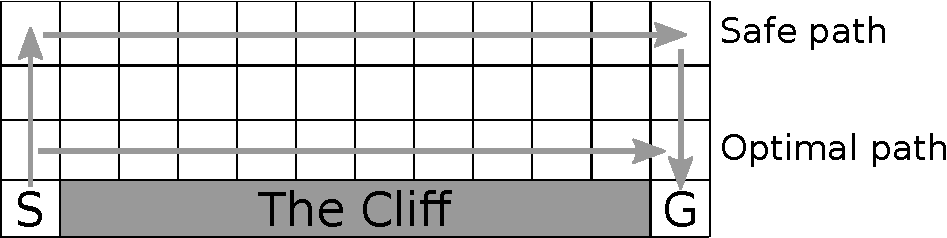
\includegraphics[width=0.5\textwidth]{figures/on_off_policy}			
	\caption{Example reward distribution for a 5-armed bandit problem.}
	\label{fig:on_off_policy}
\end{figure}

200 agents are simulated for 500 episodes to demonstrate the difference between on and off policy learning methods. They all follow \eps-greedy policies with $\epsilon=0.1$, but half use Sarsa and the other half Q-learning. The Q-learning agents learn the optimal policy and thus travel right along the edge of the cliff. However since the agents may at any point take a step into any random direction, it is better to take the safer route further away from the edge. Since the Sarsa agents learn the roundabout policy, this is the path they learn to take. Figure~\ref{fig:on_off_policy_results} show the results of these simulations.

However once the agents have been trained and \eps  is set to zero, the Q-learning agents outperform the Sarsa agents. With these new greedy policies the Q-learning agents will always receive a sum of rewards of $-12$ while the Sarsa agents receive $-16$ thanks to the longer path. If \eps  is gradually reduced to zero, then both methods converge to the optimal policy.

\begin{figure}[ht]			
	\centering
	
\includegraphics[width=0.6\textwidth]{figures/on_off_policy_results}			
	\caption{Example reward distribution for a 5-armed bandit problem.}
	\label{fig:on_off_policy_results}
\end{figure}


